\chapter{
%Modeling Animal space-usage with 
%Detection Models based on Ecological Distance
%Ecological Distance Models in Spatial Capture-Recapture
Ecological Distance in Spatial Capture-Recapture Models
}
\markboth{Chapter XXX}{}
\label{chapt.implicit}


\vspace{.3in}


%% this material is a general introduction for a manuscript
Spatial capture-recapture models are a relatively new class of models
for estimating animal density from capture-recapture data with
auxiliary information about individual capture locations (Borchers and
Efford 2008; Royle and Young 2008; Efford et al. 2009; Royle et
al. 2009).  The basic idea is to express encounter probability of
individuals as a function of the distance between individual center of
activity, say ${\bf s}_{i}$, and trap location, say ${\bf x}_{j}$.  In
these models ${\bf s}_{i}$ is regarded as a latent variable and
conventional methods of statistical inference either based on marginal
likelihood \citep{borchers_efford:2008} or Bayesian analysis by MCMC
\citep{royle_young:2008}.

While the models are a relatively recent innovation, their use is
already becoming widespread (Efford et al. 2009; Gardner et al. 2010;
Kery et al. 2010; Efford 2011; Gopalaswamy et al. 2012; Foster and
Harmsen 2012) because they resolve critical problems with using
ordinary non-spatial capture-recapture methods such as ill-defined
area sampled, heterogeneity in encounter probability due to the
juxtaposition of individuals with traps, and they provide a framework
for modeling of trap-specific covariates.  Furthermore, essentially
all real capture-recapture studies produce auxiliary spatial
information and therefore SCR models are directly relevant to standard
data collected from such studies. Indeed, the use of ordinary
capture-recapture models essentially admits a model misspecification
(i.e. homogeneous encounter probability) by ignoring the explicit
spatial information.

Every application of SCR models to this point is based on encounter 
probability models in which distance between individual activity center 
and trap location is parameterized by simple Euclidean distance.
%Previously we have only considered stationary and symmetric models for detection probability. 
While these will often be sufficient for practical purposes,
especially in small data sets, there will sometimes be interest in
developing more complex models of the detection process as it relates
to space usage of individuals.
%These models are simple because they are based on
%Euclidean distance -- which are convenient because we know this
%distance precisely conditional on individual activity center ${\bf  s}$.
However, animals may not judge distance in terms of euclidean distance
but, rather, according to quality of local habitat, landscape
connectivity and other considerations that statisticians might not
really understand. Moreover, because encounter probability and the
distance metric upon which that is based represent outcomes of
individual movements about their home range, it is natural that
landscape ecologists might have explicit hypotheses about things that
affect the distance metric.

In this section we develop models for detection probability based on
alternative distance metrics that account for ecological
considerations -- which, in keeping with the conventions in the
ecological literature, we will call ``ecological distance''. In
particular, we adopt a cost-weighted distance metric which is an idea
in widespread use in landscape ecology for modeling connectivity,
movement and gene flow
\citep{adriaensen_etal:2003,manel_etal:2003,mcrae_etal:2008}. In the
context of SCR models we can use this as the basis for computing the
distance between traps and individuals activity centers. In this way
we can explicitly accommodate some landscape structure and ideas
related to how animals use space in SCR models. We develop a
likelihood-based inference framework for SCR model parameters using
this new distance metric when the ecological distance function is
known.  We show that the MLEs are approximately unbiased in moderate
sample sizes, as expected, but also that the misspecified model based
on Euclidean distance can produce substantial bias in estimates of $N$
and hence density.  Finally, we extend the model to allow for the case
where the distance metric is only known by a covariate and the
relative ``cost'' is estimated by maximum likelihood in addition to
other encounter probability parameters and density.


\section{Spatial Capture-Recapture}

A number of distinct observation models have been proposed for
spatial-capture situations, including Poisson, multinomial or binomial
observation models. Here we focus on the binomial model in which we
suppose that $J$ traps at locations ${\bf x}_{j}$ are operated for $K$
periods (e.g., nights) although our development of cost-distance
models is directly applicable to other observation models without any
further technical considerations. The binomial model is most directly
relevant to devices such as ``hair snares'' (Gardner et al. 2010) or
scent sticks \citep{kery_etal:2010} for which individuals can only be
encountered a single time per observation occasion.

The observations are the individual- and trap specific counts $y_{ij}$
which are binomial counts with sample size $K$ and probabilities
$p_{ij}$. A standard encounter probability model (Borchers and Efford
2008) is the Gaussian model in which
\[
log(p_{ij})= \theta_{0} + \theta_{1} dist({\bf x}_{j} - {\bf s}_{i})^{2}
\]
or, equivalently, 
\[
p_{ij} = \lambda_{0} exp(-  dist({\bf x}_{j} - {\bf s}_{i})^{2}
/(2\sigma^{2}) )
\]
where $\theta_{0} = log(\lambda_{0})$ and $\theta_{1} =
-1/(2\sigma^2)$. 

In all previous applications of SCR models that appear in the
literature, encounter probability models have been based on the normal Euclidean
distance exclusively, 
i.e., $ dist({\bf x}_{j} - {\bf s}_{i}) =
||{\bf x}_{j} - {\bf s}_{i}||$,
and the parameters $\theta_0$ and $\theta_1$
have been estimated using standard methods (likelihood or
Bayesian). These methods regard ${\bf s}_{i}$ as realizations of a
point process (i.e., latent variables) and remove them from the
likelihood either under a model of ``uniformity'' in which ${\bf s}
\mbox{Uniform}({\cal S})$ where ${\cal S}$ is the state-space of the
point process, or in which covariates might affect the spatial
distribution of individuals (..... XYZ .....). Alternative detection
models are commonly used, but they are all functions of Euclidean
distance and so we do not them here. 

The critical consideration that motivates our work is that this 
 Euclidean distance metric is unaffected by habitat or landscape
structure..... and it implies that space usage of individuals is
stationary, isotropic and symmetric which may be unreasonable in most
applications. 
Subsequently we provide an extension of this class of SCR models that
accommodates alternative distance metrics that explicitly incorporate
information about the landscape so that a unit of distance is variable
depending on identified covariates. Thus, ``where'' an individual
lives on the landscape, and the state of the surrounding landscape,
will determine the character of its usage of space. In particular, we
suggest distance metrics that imply irregular, asymmetric and
non-stationary home ranges of individuals. 

\section{Cost Distance}

We use a cost-weighted distance metric in the package \mbox{\tt
gdistance} \index{R package!gdistance} which computes the distance 
between points by accumulating pixel-specific costs assigned by the user 
(but we consider estimating these in Sec. XYZ). The idea is widely used in
landscape ecology for modeling connectivity, movement and gene flow
\citep{adriaensen_etal:2003,mcrae_etal:2008}. As is customary for reasons of
computational tractability we consider a discrete landscape defined by a 
raster of some prescribed resolution. The distance between any two points 
${\bf x}$ and ${\bf x}'$ can be represented by a sequence of line segments 
connecting a sequence of neighboring  pixels say 
${\bf l}_{1},{\bf l}_{2},\ldots,{\bf l}_{m}$. Then the cost-weighted distance 
between ${\bf x}$ and ${\bf x}'$ is
\begin{equation}
 d({\bf x},{\bf x}')
  =  \sum_{i=1}^{m-1} cost({\bf l}_{i},{\bf l}_{i+1})||{\bf l}_{i} - {\bf l}_{i+1}||
\label{eq.costweighted}
\end{equation}
where $cost({\bf l}_{i},{\bf l}_{i+1})$ is the user-defined cost to move 
from pixel ${\bf l}_{i}$ to neighboring pixel ${\bf l}_{i}$ in the sequence.
In this paper we consider modeling cost as a function of covariates
defined on every pixel of the raster according to, for example using a
single
covariate $z(x)$:
\begin{equation}
 log(cost(x))=  \theta_{2} z(x) 
\label{eq.cost}
\end{equation}
Thus, if $\theta_{2} = 0$ then substituting $cost(x)$ into
Eq. \ref{eq.costweighted} will produce the ordinary Euclidean distance
between points. 
In practical applications, i.e., in landscape ecology, variables that
influence the cost of moving across the landscape include things like
distance to roads, elevation, ruggedness, human disturbance and
related things (Tabitha can you say something smart-sounding here?).

Given the ``cost'' of each pixel, it is a simple matter to compute the
cost-weighted distance between any two pixels, along {\it any} path,
simply by accumulating the intermittent costs weighted by distances. 
To be consistent with our use of the {\bf R} package \mbox{\tt
  costDistance} (REF HERE),
the incremental cost of moving from one pixel to another is the
distance-weighting of the {\it average} of the 2 pixel costs (see below).
In the context of spatial capture-recapture models (and, more
generally, landscape connectivity) we are concerned with the {\it
  minimum} cost-weighted distance between any two points.  That is, we
seek to find the 
sequence ${\bf l}_{1},{\bf l}_{2},\ldots,{\bf l}_{m}$ that minimizes
the objective function defined by Eq. \ref{eq.costweighted}.
This is done in some GIS packages and also in the {\bf R} package
\mbox{\tt costDistance} using the implementation of Dijkstra's algorithm (Dijkstra 1959)
found in the \mbox{\tt igraph} package (REF HERE).

\begin{comment}
%%%%%%%%%% As a consequence, the terminal value is not counted. 
In addition to \mbox{\tt gdistance} we use functions from a number of
other {\bf R} packages including \mbox{\tt rgeos}, \mbox{\tt
  shapefiles} and \mbox{\tt raster}.

%% Kimmy: can you look up the algorithm that Gdistance uses?  
The algorithm XYZ XYZ (REF XYZ) seeks to find the  sequence of pixels ${\bf l}_{1},
\ldots, {\bf l}_{m}$ which minimizes the cost-weighted distance. 
\end{comment}

As an example of the cost-weighted distance calculation consider the
following landscape comprised of 16 pixels with unit spacing 
identified as follows, along with the pixel-specific cost:
\begin{verbatim}
  pixel ID                 Cost
  1  2  3  4          100   1   1  1
  5  6  7  8          100 100   1  1
  9 10 11 12          100 100 100  1
 13 14 15 16          100 100   1  1 
\end{verbatim}
Then we assign low cost of 1 to ``good habitat'' pixels (or pixels we
think of as ``highly connected'' by virtue of being in good habitat)
and, conversely, we assign high cost (100) to ``bad habitat''. So the
shortest cost-weighted distance between pixels 2 and 3 in this example
is just 1 unit, the shortest cost-distance between pixels 2 and 7 is
%% Kimmy use this raster in the code below and then revise the stated
%% cost-distances
%% between the pixels
sqrt(2) units, the shortest distance between pixels 13 and 14 is 100
units, while the shortest cost-distance between 13 and 15 is 100. A
tough one is: what is the shortest distance between 10 and 16? A guy at pixel
10 can move diagonal and pay sqrt(2)*1 + 1 total.
An alternative pixel labeling scheme arising as if you were applying
the vec operation to the matrix ``as you look at it''. This produces
labels that are a transpose of those given previously, so the id's are
as follows:
\begin{verbatim}
 1 5  9 13
 2 6 10 14
 3 7 11 15
 4 8 12 16
\end{verbatim}
In this case we have to transpose or rotate something along the way. 
Be careful. This matters in the way you stick the ``cost'' data into
the elements of the raster.
In the following example we fill the cost
matrix using the default \mbox{\tt byrow=FALSE} standard in {\bf
  R}, but here we use cost values of 1-16 so that we can produce an
image of the resulting costs to visualize their ordering in the raster:
\begin{verbatim}
r<-raster(nrows=4,ncols=4)
projection(r)<- "+proj=utm +zone=12 +datum=WGS84"
extent(r)<-c(.5,4.5,.5,4.5)
values(r)<-matrix(1:16,4,4,byrow=FALSE)
par(mfrow=c(1,1))
plot(r)
\end{verbatim}
The raster, in image form, is shown in Fig. \ref{ecoldist.fig.raster}.

\begin{figure}
\begin{center}
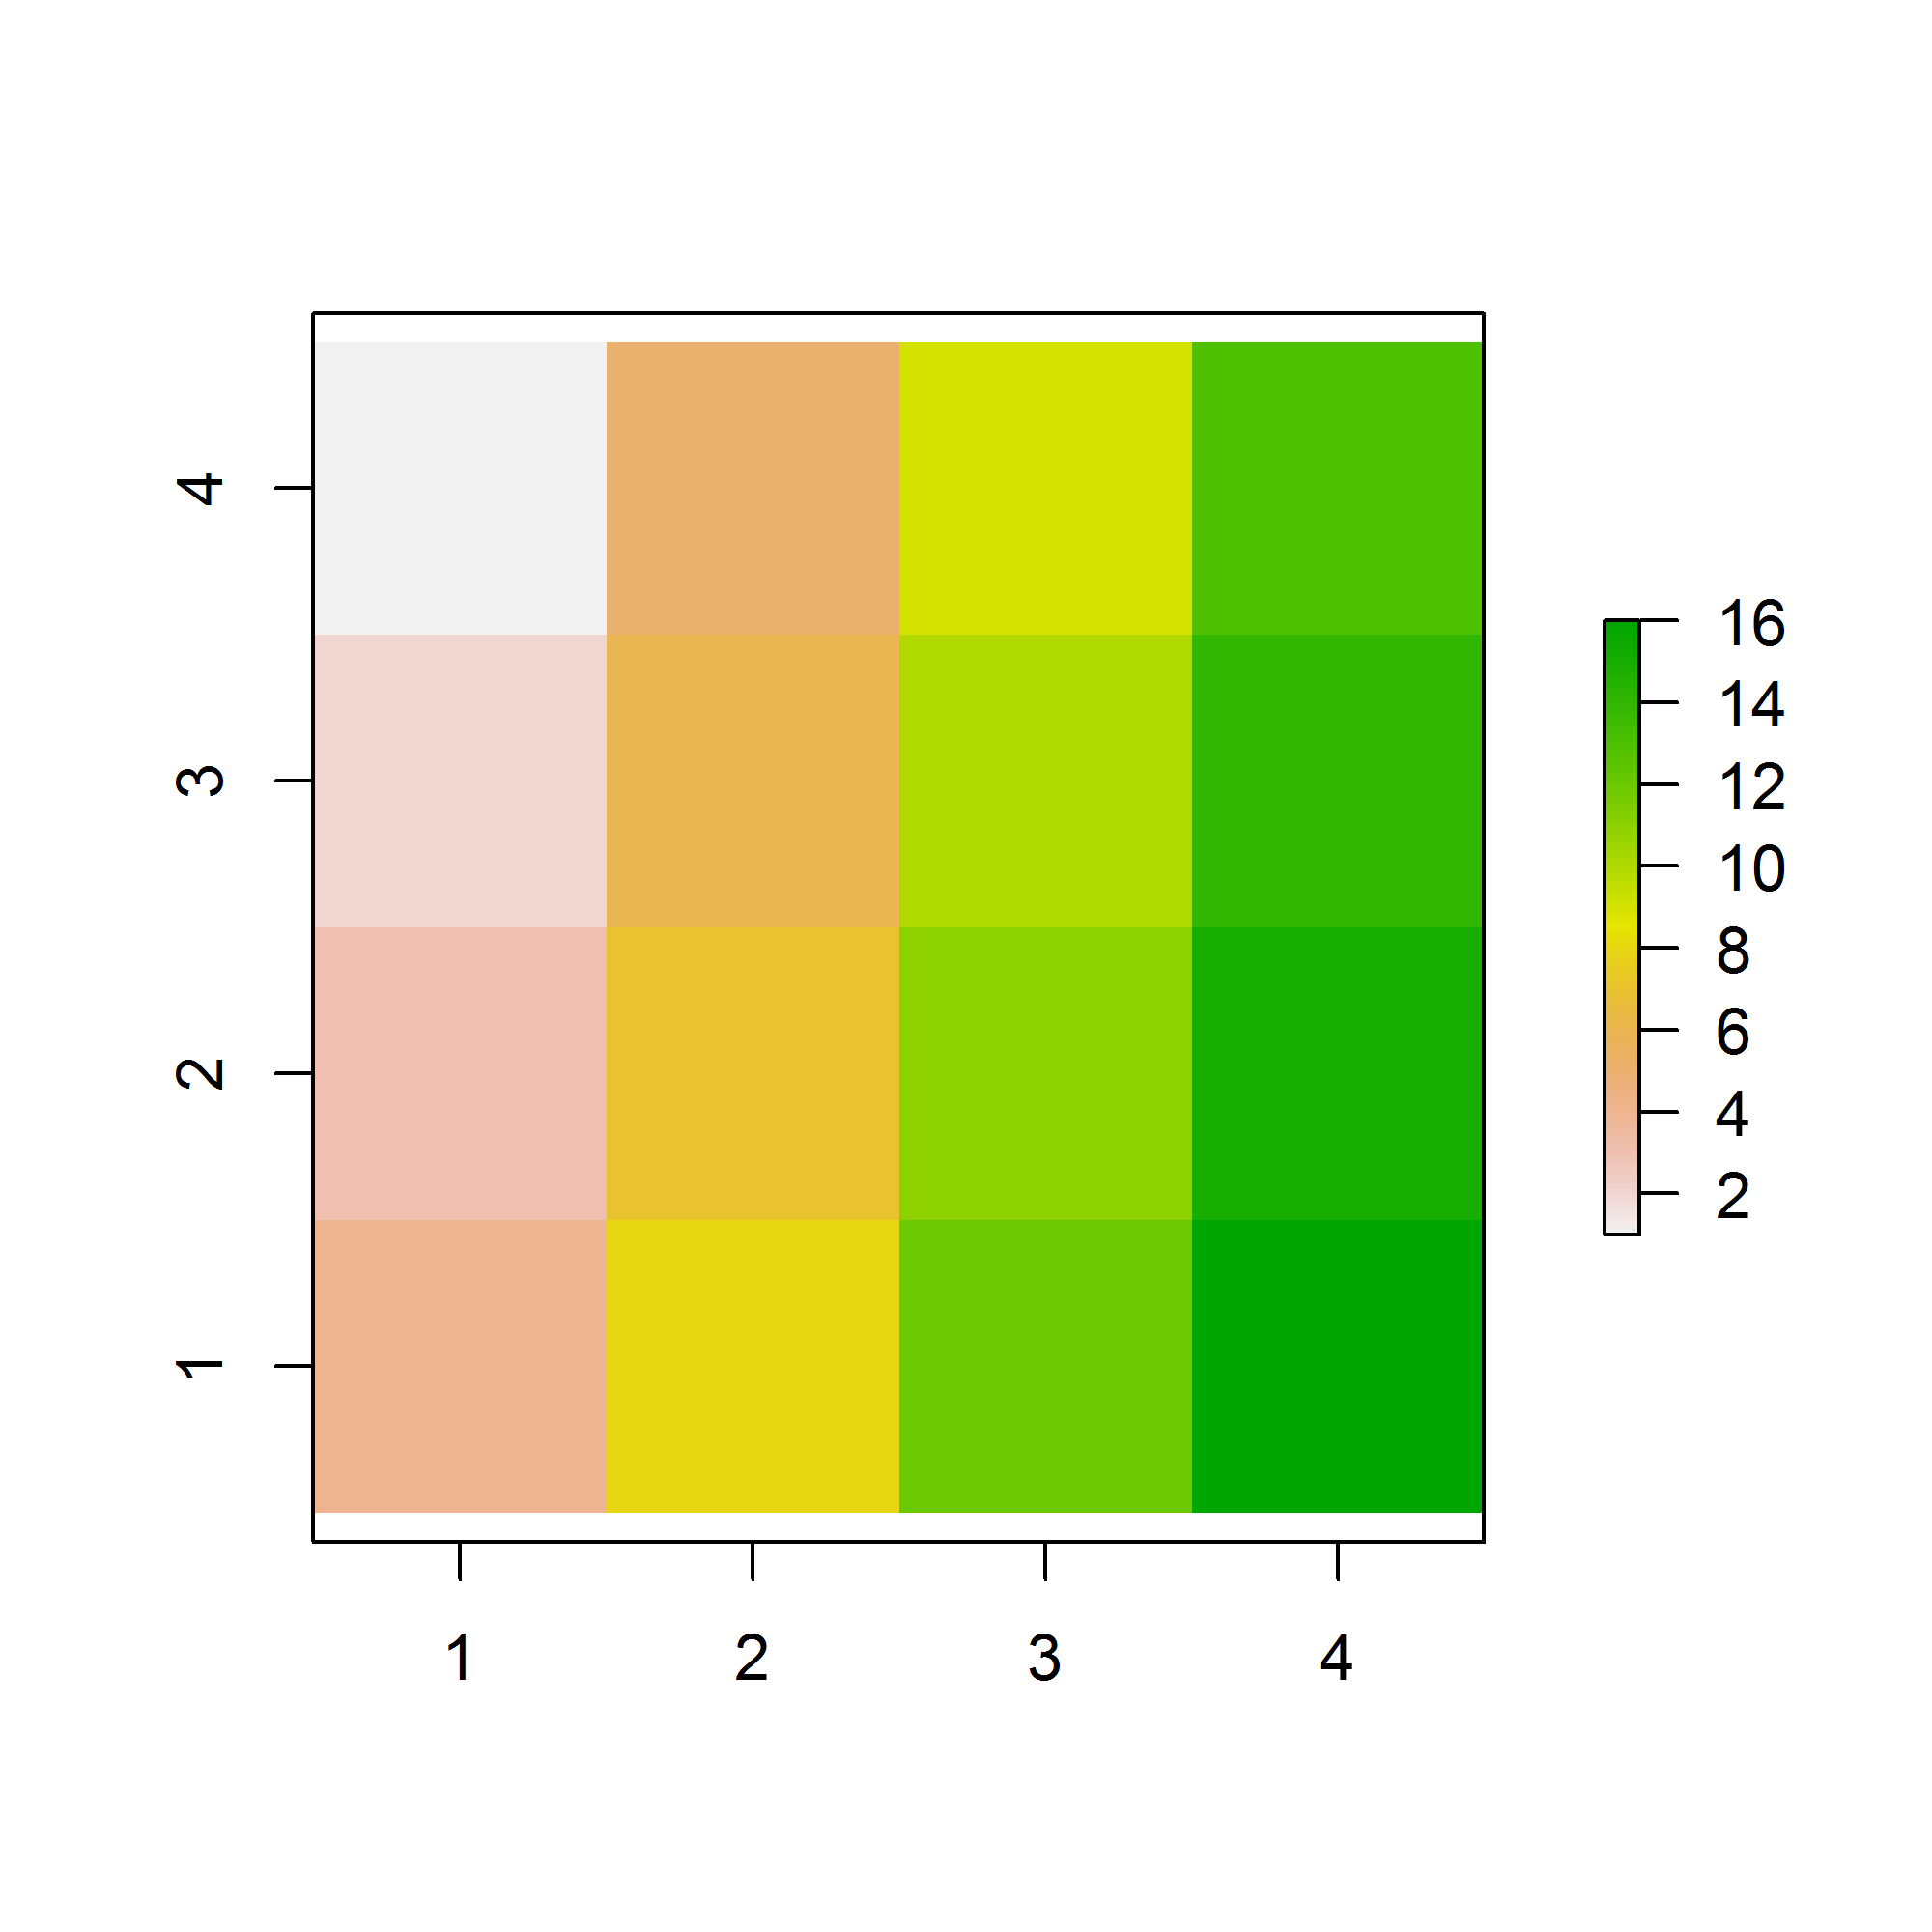
\includegraphics[height=3.25in,width=3.25in]{Ch10/figs/raster}
\end{center}
\caption{a 16 pt raster}
\label{ecoldist.fig.raster}
\end{figure}

Then we use the functions \mbox{\tt transition}, \mbox{\tt
  geoCorrection} (which doesn't really do anything but reformat the
data somehow) and \mbox{\tt costDistance} to compute the distance
matrix. They operate on this inverse-scale so we first take the 
element-by-element inverse of the raster. Then we define a set of points,
the center points of each raster, to compute the cost-distance between
them all. The commands altogether are as follows:
\begin{verbatim}
tr1<-transition(r,transitionFunction=max,directions=8)
tr1CorrC<-geoCorrection(tr1,type="c",multpl=FALSE,scl=FALSE)
tr1CorrC<-1/tr1CorrC  # because the transitions are computed in conductance which is 1/cost
pts<-cbind( sort(rep(1:4,4)),rep(4:1,4))
costs1<-costDistance(tr1CorrC,pts)
outD<-as.matrix(costs1)
\end{verbatim}
Now we can look at the result and see if it makes sense to us. Here we
print the first 4 columns of this distance matrix and illustration a
couple of examples of calculating the minimum cost-weighted distance
between points:
\small{
\begin{verbatim}
> outD[,1:4]
      1    2    3    4
1   0.0  1.5  4.0  7.5
2   1.5  0.0  2.5  6.0
3   4.0  2.5  0.0  3.5
4   7.5  6.0  3.5  0.0
5   3.0  4.5  7.0 10.5
6   5.5  4.0  6.5 10.0
7   9.0  7.5  5.0  8.5
8  13.5 12.0  9.5  6.0
9  10.0 11.5 14.0 17.5
10 13.5 12.0 14.5 18.0
11 18.0 16.5 14.0 17.5
12 23.5 22.0 19.5 16.0
13 21.0 22.5 25.0 28.5
14 25.5 24.0 26.5 30.0
15 31.0 29.5 27.0 30.5
16 37.5 36.0 33.5 30.0
\end{verbatim}
}
{\bf NEED TO REVISE BELOW}
Moving down the first (left-most, as you look at it) column of the
raster the cost-distance between pixel 1 and 2 is 1.0 which we know to
be right because the cost of leaving pixel 1 is tabulated, and that is
the value 1.0.  To get from pixel 1 to pixel 3 we have to leave both
pixels 1 and 2, for a total cost of $1+2 = 3$ which is the result
given above.  To see that the shortest cost-weighted distance is not always the
shortest Euclidean distance, consider moving from pixel .....



\section{Maximum likelihood estimation}

Here we develop a standard method of parameter estimation based on
the marginal likelihood. That is, the likelihood in which the latent
variables ${\bf s}$ are removed by integration (Borchers and
Efford 2008). 

The individual- and trap-specific observations have a binomial
distribution conditional on the latent variable ${\bf s}_{i}$:
\begin{equation}
	y_{ij}| {\bf s}_{i} \sim \mbox{Bin}(K, p_{\theta}({\bf x}_{j},{\bf s}_{i}))
\label{mle.eq.cond-on-s}
\end{equation}
where we have indicated the dependence of $p_{ij}$ on ${\bf s}$ and
the vector of parameters ${\bm \theta}$ explicitly. The parameters
${\bm \theta}$ include whatever parameters are involved in the
cost-weighted distance function, i.e., at least $\theta_{2}$ from 
Eq. \ref{eq.cost}.
For the random effect we have ${\bf s}_{i} \sim  \mbox{Unif}({\cal
  S})$.
The joint distribution of the data for individual $i$ is the product
of $J$ binomial terms (i.e., contributions from each of $J$ traps):
\[
  [{\bf y}_{i} | {\bf s}_{i} , \theta] = 
  \prod_{j=1}^{J} \mbox{Bin}(K, p_{\theta}({\bf x}_{j},{\bf s}_{i}) )
\]
This assumes that encounter of individual $i$ in each
trap is independent of encounter in every other trap. Conditional on
${\bf s}_{i}$ this is reasonable in most applications in our view.
 The so-called marginal likelihood is computed by removing
${\bf s}_{i}$, by integration,  from the conditional-on-${\bf s}$
likelihood and regarding the {\it marginal} distribution of the data
as the likelihood. That
is, we compute:
\[
  [y|\theta] = 
\int_{{\cal S}}  [ \theta | {\bf y}_{i} |{\bf s}_{i}] g({\bf s}_{i}) d{\bf s}_{i}
\]
where, under the uniformity assumption, we have
$g({\bf s}) = 1/||{\cal S}||$.
The joint likelihood for all $N$ individuals, assuming independence of
encounters among individuals, is the product of $N$ such terms:
\[
{\cal L}(\theta | {\bf y}_{1},{\bf y}_{2},\ldots, {\bf y}_{N}) = \prod_{i=1}^{N}
[{\bf y}_{i}|\theta]
\]

The key operation for computing the likelihood is solving the
2-dimensional integration problem to remove ${\bf s}$. There are some
general purpose {\bf R} packages that implement a number of
multi-dimensional integration routines including \mbox{\tt adapt}
\citep{genz_etal:2007} and \mbox{\tt R2cuba} \citep{hahn_etal:2011}.
We won't rely on these extraneous {\bf R} packages but instead will
use perhaps less efficient methods in which we replace the integral
with a summation over an equal area mesh of points on the state-space
${\cal S}$ and explicitly evaluate the integrand at each point. We
invoke the rectangular rule for integration here in which the
integrand is evaluated on a regular grid of points of equal area and
then averaged.  Let $u=1,2,\ldots,nG$ index a grid of $nG$ points,
${\bf s}_{u}$, where the area of grid cell $u$ is constant.  In this
case, the integrand, i.e., the marginal pmf of ${\bf y}_{i}$, is
approximated by
\begin{equation}
         [{\bf y}_{i}|\theta] = \frac{1}{nG} \sum_{u=1}^{nG}  [ {\bf
            y}_{i} |{\bf s}_u, \theta]
\label{mle.eq.intlik}
\end{equation}

To deal with the fact that $N$ is unknown, 
there are two key issues that need to be addressed.
First is that 
we don't observe the all-zero encounter history so we have to
make sure we compute the probability for that ``all zero'' encounter history which
we do operationally by tacking a row of zeros onto the encounter history matrix. In
addition, we include the number of such all-zero encounter histories
as an unknown parameter of the model. Call that unknown quantity $n_{0}$.
In addition, we have to be sure to include a combinatorial term to
account for the fact that of the $n$ observed individuals there are
${N \choose n}$
 ways to realize a sample of size $n$. The combinatorial term
involves the unknown $n_{0}$ and thus it must be included in the likelihood.

To compute the integral requires that the bounds of integration are
specified, which is equivalent to prescribing the state-space of the
underlying point process, i.e., ${\cal S}$. Therefore density is
computed as $D({\cal S}) = N/||{\cal S}||$. In our simulation study
below we report $N$ as the two are equivalent summaries of the data
set once the state-space is fixed. 

We wrote an R function to evaluate the likelihood which we optimize
using the R function \mbox{\tt nlm}.
The R code is given as a script in the Appendix and the R package scr
is available on the website XYZ along with functions for simulating
data.


\section{Examples of Computing Cost-Distance}

In this section we provide an example that we think is typical of 
how cost-weighted distance models can be used in real
capture-recapture problems.

\begin{comment}
In particular, we will typically have a polygon coverage either in the
form of a GIS shapefile or a matrix of points or some other specific
format, and we want to put that polygon on a map and use the polygon
boundary in some way to generate pixel-specific costs. So we want to
see if points or raster pixels are in the polygon, or not, or how far
they are from the polygon boundary (cost might be related to distance)
and similar operations. In the following examples, we confront how to
do some of these operations in {\bf R}. 
\end{comment}

We develop an example here using a $20 \times 20$ pixel raster with
extent $[0.5, 4.5] \times [0.5, 4.5]$.
We regard for the purposes of this example as a coarse landscape 
covariate, with (scaled) pixels having ,  say, a $2 \times 2$ km resolution. Thus, the raster
therefore
defines a landscape of $40 \times 40$ km and we suppose that 16 camera
traps are established at the integer coordinates (1,1), (1,2),
... (4,4). 
Maybe we are studying a population of ocelots or lynx or some other
spotted cat.
We suppose 
that each raster is characterized by a single covariate which is increasing 
from the NW to the SE. This might define something related to distance
from an urban area or a gradient in habitat quality due to land use,
or environmental conditions. 
We define 
\[
 log(cost(x))=  \beta z 
 \]
where $\beta = 1$ which we regard as known. With $\beta=0$ then the model reduces to
one in which the cost of moving across each pixel is constant, and therefore Euclidean
distance is operative.
 Of course this is a model and it is completely
unreasonable to regard $\beta$ as known but this is standard practice in essentially all
historical studies of landscape or genetic connectivity although sometimes crude methods
of estimation in specific contexts are based on comparing distance matrices of genetic
structure with those produced by simulation models so that either $\beta$ might be estimated
crudely or covariates which improve fit can be selected. REFs????
However this stuff has never been formalized in a likelihood context and especially
not for SCR models. 
Anyhow, we consider the known-$\beta$ situation first before dealing with estimating
this parameter. 


\subsection{Simulation studies}

We devised a limited simulation study to evaluate three things: (1)
the general statistical performance of the density estimator under
this new model; (2) the effect of mis-specifying the model with a
normal Euclidean distance metric and (3) the statistical performance
of estimating the relative cost parameter.

We used population sizes of 100 and 200 individuals and subjected them
to encounter by 16 traps arranged in a $4\times 4$ grid according to
the Euclidean distance metric. We fit 3 different models; (i) the
misspecified euclidean distance model; (ii) the true data-generating
model with the relative cost raster {\it known} and (iii) the true
data-generating model but estimating the relative cost parameter by
maximum likelihood.  A sample realization of this is shown in Fig.
\ref{ecoldist.fig.raster100}.

We simulated a few levels of N and detection probability 
hi p: alpha0<- -2     sigma<- .5    K<-10
lo p: alpha0<- -2     sigma<- .5    K<- 5
Because any simulation study is inherently arbitrary, we have provided R scripts
for carrying out simulations in the Appendix so that the interested reader can experiment with
their own situations.

\begin{figure}
\begin{center}
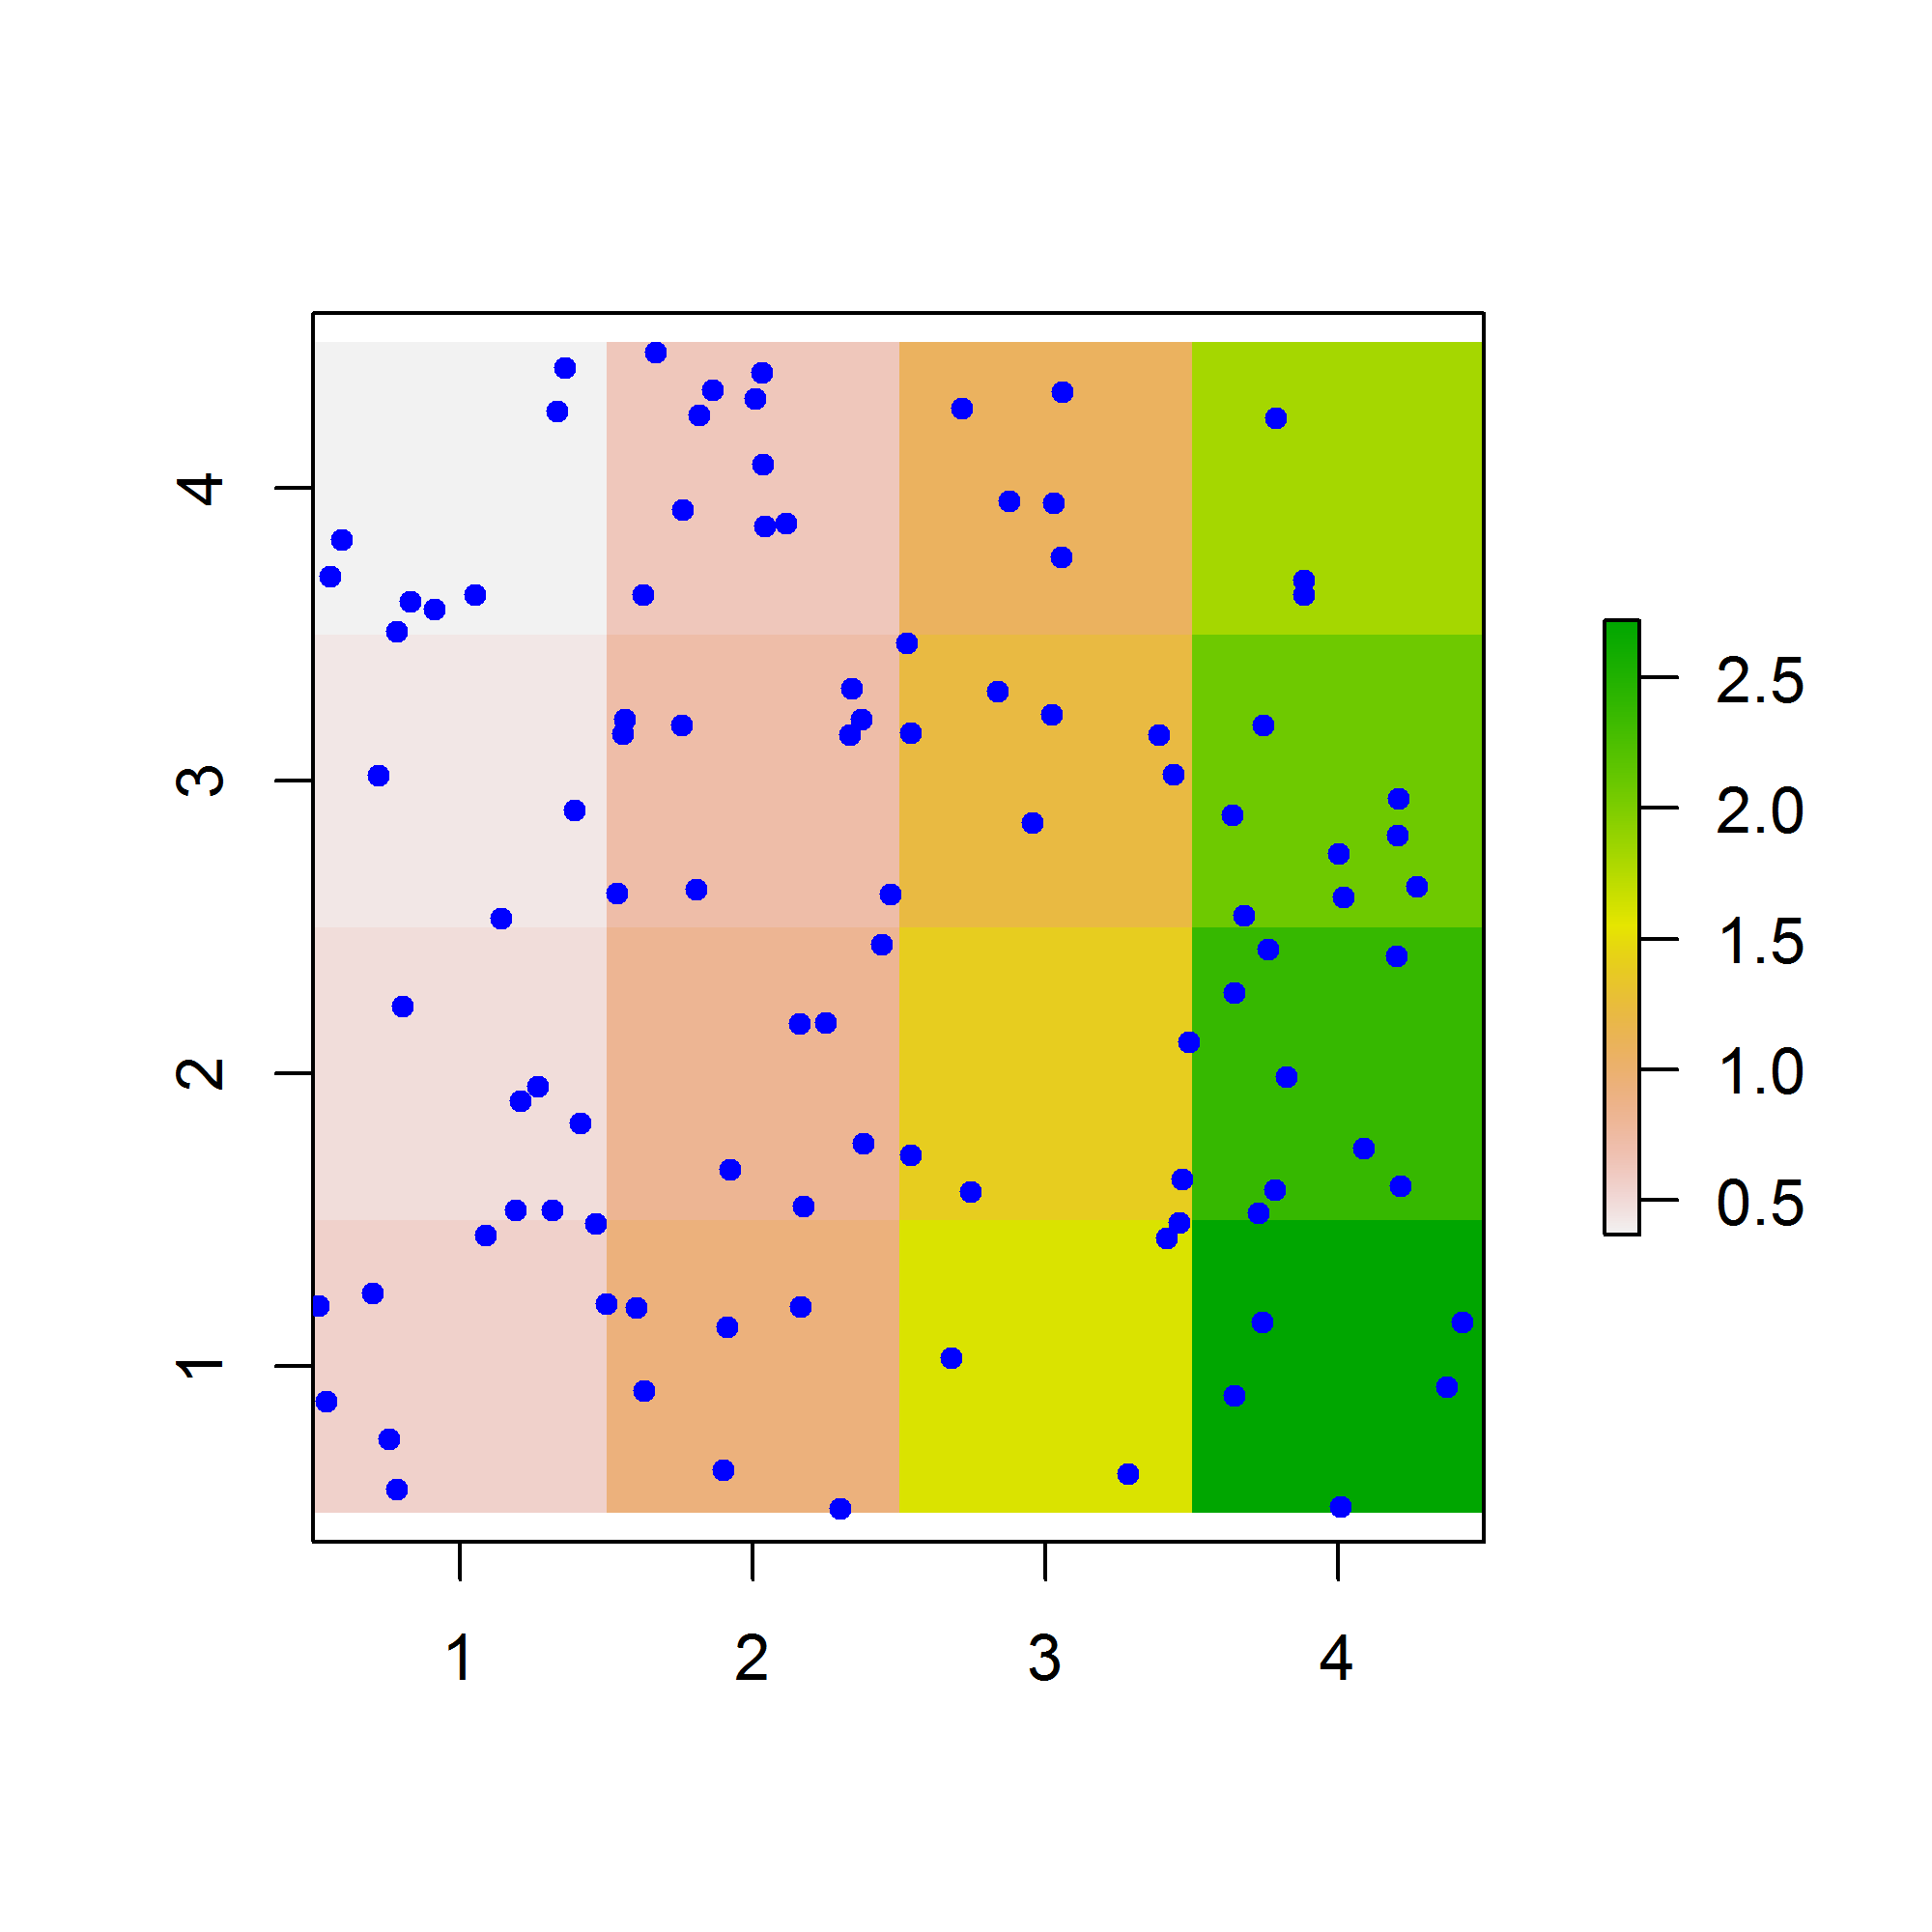
\includegraphics[height=3.25in,width=3.25in]{Ch10/figs/raster_withN100}
\end{center}
\caption{a 16 pt raster with 100 guys living on it}
\label{ecoldist.fig.raster100}
\end{figure}
 


\begin{verbatim}
Summaries of sampling distribution
             mean         SD        0.025       0.50     0.975
high p cases  
N=100      mean n = 84.6
euclid      92.206114   4.671663  83.805619  91.992918 101.062115 
ecol/known  98.968879   4.664292  89.364618  99.263953 107.489414 
ecol/est    99.078592   4.718402  89.381868  99.569445 107.767255 
N=200
euclid     185.195251   5.508866 176.687894 184.911376 195.955084 
ecol/known 198.682523   5.578265 189.409647 197.983286 209.565110 
ecol/est   199.032216   5.832957 189.098127 198.821324 210.572747 

low p cases  mean n = 64.5 
N=100
euclid      90.53286  10.78777  71.70875  88.98319 111.13541 
ecol/known 100.64718  10.89509  78.66732 100.85660 122.05896 
ecol/est   101.18081  11.26187  77.01104 101.54720 122.75944 

\end{verbatim}

20 x 20 raster with trend
\begin{verbatim}
N=100    E[n] = 50.89
euclid       64.782766  6.970634 50.988559 64.064815 77.018504 
ecol/known   96.54721  11.84963  74.34012  97.51291 118.48684 
ecol/est     98.40953  13.10363  73.10170  99.96509 124.97876 
\end{verbatim}


\section{Discussion}

Interest in SCR models has grown rapidly in the last several years
since their formalization using likelihood (Borchers and Efford 2008)
and Bayesian (Royle and Young 2008) inference methods. This is because
of both the severe practical limitations of classical non-spatial
capture-recapture models, and also the ubiquity of auxiliary spatial
information in all capture-recapture studies, and thus the universal
applicability of SCR models.

All applications of SCR models have been based on models for the
encounter probability that use the standard Euclidean distance between
individuals and traps. This has obvious limitations that it is
unaffected by landscape or habitat structure and it implies
stationary,  isotropic and symmetrical home ranges. These are standard
criticisms of the basic SCR model as universally applied in practice. 
In this paper,  we have developed for the first time a formal framework for integrating
``ecological distance'' into SCR models, where ecological distance is
defined as a cost-weighted distance between points, and where ``cost''
is characterized by one or more spatially explicit covariates that are
believe to influence movement or space-usage of individuals.  


How animals use space and therefore how distance to a trap is
perceived by individuals is not something that can ever be known. We
can only ever conjure up models to describe this
phenomenon. Historically we have come up with models and had to regard
those as fixed up to a single parameter or two that is invariant to
the underlying landscape. Here we have shown that there is hope to
estimate parameters, from capture-recapture data,
 that describe how animals use space and thereby
allowing for irregular home range geometry that is influenced by
landscape structure, and resulting affect on encounter probability in
the context of capture-recapture studies. 

As expected, our simulation study demonstrated that the MLE of model
parameters is approximately unbiased in moderate sample
sizes. Moreover, the 
effect of ignoring ecological distance and using normal Euclidean
distance in the model for encounter probability, has the 
logical effect of causing negative bias
in estimates of $N$. We expect this because the effect is similar to
failing to model heterogeneity. i.e., if we misspecify ``model Mh'' with
``Model M0'' then we will expect to under-estimate $N$. So the effect of
mis-specifiying the ecological distance metric with a standard
homogeneous euclidean distance has the same effect.

In our view, this bias is not really the most important reason to consider models of
ecological distance. Rather, inference about the structure of
ecological distance is fundamental to many problems in applied and
theoretical ecology that have to do with modeling landscape
connectivity, corridor and reserve design, population viability
analysis, gene flow, and other phenomena. 
Because encounter rate in traps, as it relates to distance from
individual activity centers, should be related to landscape
connectivity, our method allows investigators to to evaluate landscape
factors that influence movement of individuals over the landscape and
therefore SCR models based on ecological distance metrics might aid in
corridor design and understanding other aspects of space usage and
movement in animal populations. 

We adopted a standard approach to inference under our model based on
marginal likelihood (Borchers and Efford 2008). In principle, 
Bayesian analysis does not pose any unique challenges for this new
class of models, except that computing the cost-weighted distance is
computationally intensive. 
 So, having to do this at each iteration of an
MCMC algorithm may be impractical using existing algorithms.
A related issue is that the size of the raster slows things down. For
huge rasters, even likelihood analysis can be computationally challenging.

Some extensions of this method may be of interest. Instead of 
having explicit covariates it might be possible to estimate the 
``resistance surface'' as a latent field, much as \citep{wikle:2003}
 did in the developing of models of species spread based on a
 diffusion process. He define the spatially-explicit rate of 
diffusion, $\delta(x)$, as a Gaussian spatial process and it was
estimated from the data.  The coolness of this would defy experience. 















\begin{comment}

% below stuff is for the book




\subsection{Illustration: Example Good vs. Bad habitat}

Here we analyze the cost-weighted distance for a landscape created to
mimic
a habitat corridor or park unit or some other block of
relatively homogeneous good-quality habitat for some species
(Fig. \ref{ecoldist.fig.corridor}).
It is surrounded by a suburban wasteland of McDonalds and Wal-Marts, much
less hospital habitat for most things. See
We describe the steps for creating this landscape shortly, so that the
reader can use a similar process to generate more relevant landscapes
for their own problems. 

In practice, we have a landscape with multiple polygons delineating
good or bad habitat or a forest preserve or corridors or
whatever. These exist maybe as shapefiles.
We have to create a raster, overly the polygon and assign values
depending on whether pixels are in good polygons or not.
You can do this in GIS but we do a version of this in R here. See
chapter 5.XYZ for an example of reading in the shapefile and doing it.

We provide 
 a function \mbox{\tt make.seg} which allows the user to make a specific
buffer given a trap region.  You can plot the region with a range or a
specific set of points and then click over it using these commands:
{\small 
\begin{verbatim}
make.seg<-function(npts){
l2<-locator(npts)
l2<-cbind(l2$x,l2$y)
l2<-round(l2,2)
tmp<-NULL
for(i in 1:nrow(l2)){
tmp<-paste(tmp,l2[i,1],l2[i,2])
if(i<nrow(l2))
tmp<-paste(tmp,",")
}
l2b<- paste("LINESTRING(",tmp,")")
l2<- readWKT(l2b)
return(l2)
}


plot(NULL,xlim=c(0,10),ylim=c(0,10))
l1<-make.seg(9)
plot(l1)
l2<-make.seg(5)
plot(l1)
lines(l2)
\end{verbatim}
}

We used this function to create a couple of line segments of class XXX
from package xyz XXXXXX  which can be loaded as 
follows\footnote{how to put this in the R package?}:
\begin{verbatim}
load("polygons.RData")
\end{verbatim}
This has 2 polygon files in it ......representing different segments
of this corridor or river system. We use the commands XYZ to join and
buffer the two segments and the resultt is that shown in fig. XYZ.

\begin{verbatim}
buffer<- 0.5
l1<-l1.old
l2<-l2.old
par(mfrow=c(1,1))
aa<-gUnion(l1,l2)
plot(gBuffer(aa,width=buffer),xlim=c(0,10),ylim=c(0,10))
pg<-gBuffer(aa,width=buffer)
pg.coords<- pg@polygons[[1]]@Polygons[[1]]@coords

xg<-seq(0,10,,30)
yg<-seq(10,0,,30)

delta<-mean(diff(xg))
pts<- cbind(sort(rep(xg,30)),rep(yg,30))
points(pts,pch=20)

in.pts<-point.in.polygon(pts[,1],pts[,2],pg.coords[,1],pg.coords[,2])
points(pts[in.pts==1,],pch=20,col="red")

\end{verbatim}

\begin{figure}
\begin{center}
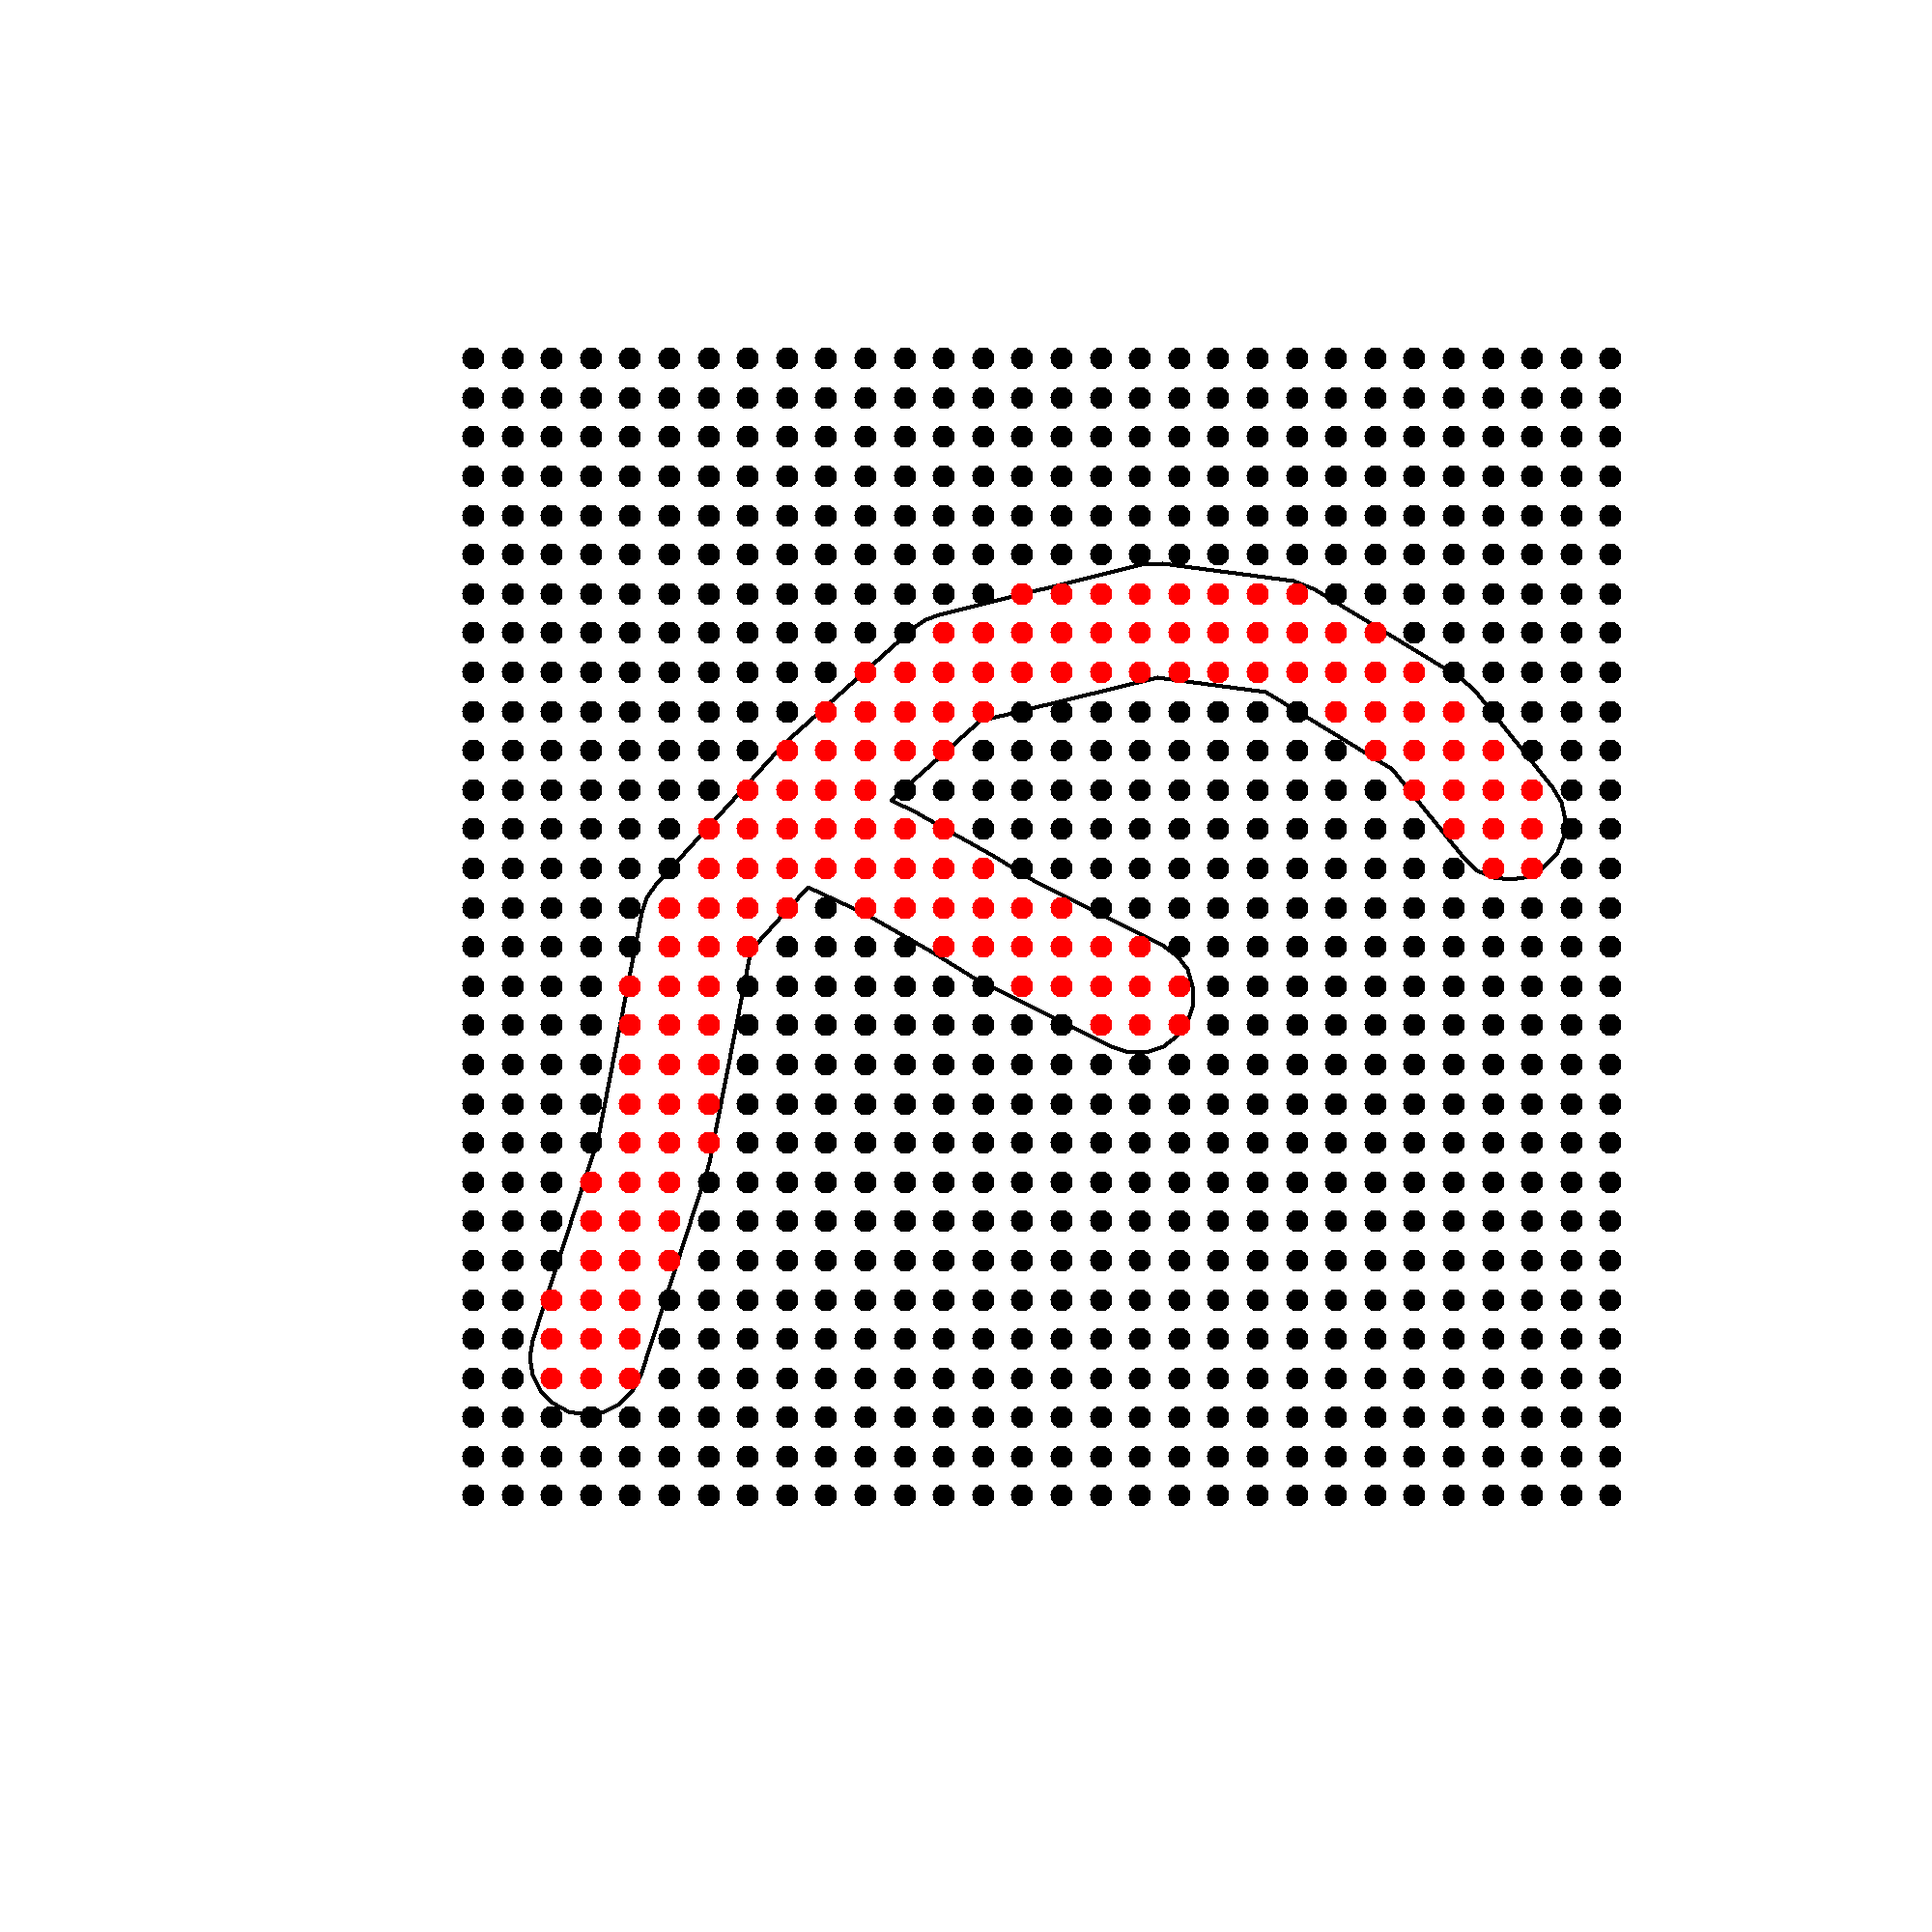
\includegraphics[height=3.25in,width=3.25in]{Ch10/figs/corridor}
\end{center}
\caption{a habitat corridor or preserve}
\label{ecoldist.fig.corridor}
\end{figure}


We focus on devising a SCR model for this corridor system and we
imagine that animals will tend to severely avoid leaving the buffered
habitat zone.

\subsection{Distance Weighting}

We consider a situation here in which we develop weights based on the
distance from some feature such as a highway or a river. 

\subsection{Hard Boundary}

\section{Ecological distance in SCR models}

Code for fitting the basic model  with minimum cost-distance {\it fixed}.



\section{Real example}


\section{Estimating Cost or Resistance Values}

\section{Bayesian Analysis}

Some of this stuff can be done easily enough in BUGS or we can code
our own. e.g., we only need the distance matrix computed ahead of time
and we can work on that with a discrete raster.  continuous space is
less easy because BUGS doesn't have a function for computing
ecological distance between any arbitrary points. 

As for estimating the parameters of the ecological distance function
-- this might at the present time be impossible in the BUGS
variants. However, we can use the functions described above to
implement our own MCMC algorithm following the developments of
Chapt. \ref{chapt.mcmc}.


\section{Summary and Outlook}

This shit is hot. We are the man. There is no limit to what we can do.


The effect of ignoring ecological distance e.g. if that is the true
data generating model would be useful to investigate for some specific
situations. obviously this will depend on the complexity of the
landscape being considered and the actual manner in which animals use
space, i.e., how they perceive distance. Since we can never know this,
any kind of sim study would be inherently arbitrary and so we didn't
pursue that here. [i guess i mean we never ever can observe actual
costs at the pixel level or even get directinfo about that because we
only observe the total distance traveled -- and that is only observed
imperfectly -- so getting direct info about cost seems difficult and
maybe not even possible. 
If we had radio-colared guys we could estimate 1st order transition
probabilities. i.e., Pr(goes to v(t+1) given at v(t)) and it seems
like those transition probabilites are direct information about cost
or propensity to go from v(t) to v(t+1).


moving around in a buffer or on a stream network seems like a useful
problem. what if we have such a network, then how screwed are we?

\end{comment}

